\documentclass[12pt,letterpaper,onecolumn]{report}
\usepackage[utf8]{inputenc}
\usepackage{amsmath}
\usepackage{amsfonts}
\usepackage{amssymb}
\usepackage{amstext}
\usepackage{amsthm}
\usepackage{graphicx}
\usepackage{exscale}
\usepackage[mathscr]{eucal}
\usepackage{bm}
\usepackage{eqlist}
\usepackage[usenames, dvipsnames]{color}
\DeclareGraphicsExtensions{.pdf, .jpg}
\newcommand{\harpoon}{\overset{\rightharpoonup}}

\usepackage{hyperref}
\usepackage{esint}
\usepackage{mathtools}
\usepackage{colortbl}
\usepackage{color}
\usepackage[utf8]{inputenc}

\usepackage[left=1in,right=1in,top=1in,bottom=1in]{geometry}

\usepackage{enumitem}
\usepackage{fancyhdr}
\pagestyle{fancy}
%\fancyhf{}
\lhead{\textbf{Lab 3}}
\chead{\textbf{ENGR 3230: Analog Circuit Design}}
\rhead{10 pts}


\begin{document}

\begin{center}
\LARGE{\textbf{Lab 3: Fuzz Face}}\\
\Large{Due: Tuesday 02/19/2019}
\\

\end{center}

\section*{Objectives}
\begin{enumerate}
\item To understand the analysis of a transistor amplifier circuit
\item To build and test a transistor amplifier circuit
\item To design, implement and test PCB circuits
\end{enumerate}

\section*{Procedure}
\subsection*{Week 1}
\begin{itemize}
\item Read the Fuzz Face Analysis found at \url{https://www.electrosmash.com/fuzz-face}
\item With the values shown, confirm the bias points specified by calculation
\item Build an LTspice model of the circuit, using the 2N2907 pnp transistor as shown below.
\item Run a DC operating point analysis using the .op command.
\item Run a transient analysis using the .tran command.  Do so for a few frequencies and a few amplitudes.  Document your trials through screen shots and in your lab notebook.
\item Build the circuit.
\item Test bias points and record data.
\item Test AC operation in the same way that you did in LTspice and document the results.
\item Try replacing the silicon transistors with germanium.  How does this impact the results?  Record your observations.
\item Test the operation of the circuit with the guitar and amplifier provided.  Adjust the values of R1, R2, and R3 until you are happy with the sound.
\item Design and mill a PCB for this circuit for next week.
\end{itemize}

\begin{center}
\begin{figure}[!h]
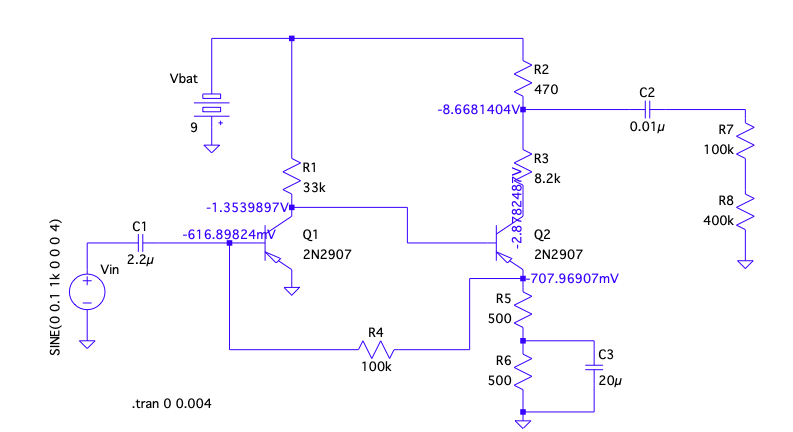
\includegraphics[width=0.9\textwidth]{Figures/fuzzface.png}
\end{figure}
\end{center}
\subsection*{Week 2}
\begin{itemize}
\item Populate your PCB.
\item Test your PCB and verify its operation through all the means for week 1.
\item Document all tests and design procedure in your lab notebook
\end{itemize}





\noindent  Submit a lab notebook (one per group) that documents all analysis, measurement, and test procedures and results.  You should include in the notebook screen shots of simulation and your PCB layout.  This lab notebook can be physical or digital.


\end{document}
